\section{PHÂN TÍCH VÀ THIẾT KẾ HỆ THỐNG}\label{sec:phan_tich_thiet_ke}

\subsection{Phân tích các sơ đồ mạng}

Trong phần này, chúng ta sẽ phân tích chi tiết hai mô hình mạng chính: Mô hình mạng phẳng (Flat Network) và Mô hình mạng phân tầng 3 lớp (Three-Tier Network). Mỗi mô hình có những ưu điểm và nhược điểm riêng, phù hợp với các môi trường và yêu cầu khác nhau.

\subsubsection{Sơ đồ mạng phẳng (Flat Network)}

\begin{figure}[H]
    \centering
    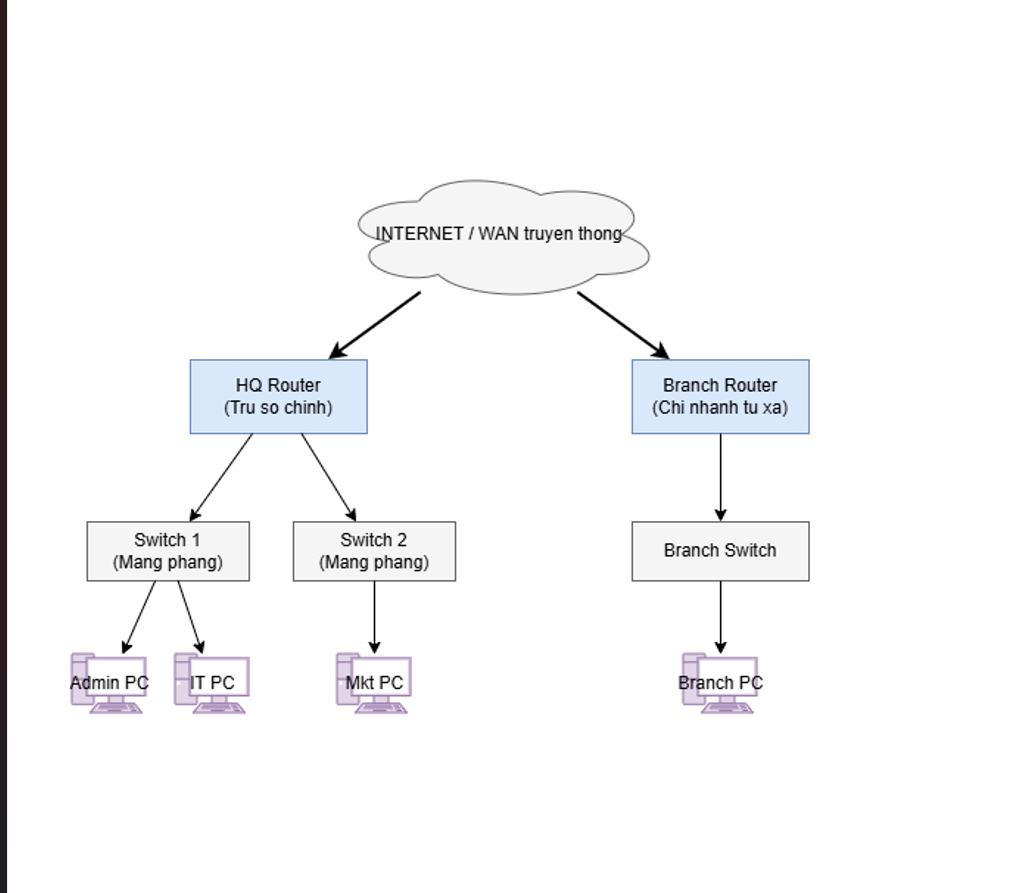
\includegraphics[width=0.9\textwidth]{image/flat_network.png}
    \caption{Sơ đồ mô hình mạng phẳng}
    \label{fig:flat_network_ch3}
\end{figure}

\paragraph{Đặc điểm cấu trúc}
Mạng phẳng là kiến trúc mạng đơn giản nhất, trong đó tất cả các thiết bị được kết nối trong cùng một broadcast domain, không có sự phân chia theo các tầng hoặc vùng mạng.

\textbf{Các thành phần chính:}
\begin{itemize}
    \item Tất cả thiết bị nằm trong cùng một subnet và VLAN
    \item Không có sự phân cấp giữa các thiết bị mạng
    \item Broadcast traffic được truyền đến toàn bộ mạng
    \item Cấu hình đơn giản, chi phí thấp
\end{itemize}

\paragraph{Ưu điểm}
\begin{enumerate}
    \item \textbf{Chi phí thấp:} Không cần đầu tư nhiều thiết bị chuyên dụng, phù hợp với ngân sách hạn chế.
    \item \textbf{Cấu hình đơn giản:} Dễ dàng triển khai và bảo trì, không yêu cầu kiến thức chuyên sâu về mạng.
    \item \textbf{Dễ quản lý:} Với số lượng thiết bị ít, việc quản lý và xử lý sự cố tương đối đơn giản.
    \item \textbf{Thời gian triển khai nhanh:} Không cần cấu hình phức tạp, có thể đưa vào sử dụng nhanh chóng.
    \item \textbf{Tương thích tốt:} Hầu hết các thiết bị đều có thể hoạt động trong môi trường mạng phẳng.
\end{enumerate}

\paragraph{Nhược điểm}
\begin{enumerate}
    \item \textbf{Hiệu năng kém khi mở rộng:} Khi số lượng thiết bị tăng lên, broadcast storm gây quá tải mạng, làm giảm băng thông khả dụng và tăng độ trễ.
    \item \textbf{Bảo mật yếu:} Không có sự phân đoạn mạng, tất cả thiết bị có thể giao tiếp trực tiếp với nhau, khó kiểm soát truy cập và dễ bị tấn công lan truyền.
    \item \textbf{Khó quản lý khi mở rộng:} Khi mạng mở rộng, việc theo dõi và xử lý sự cố trở nên phức tạp, không thể áp dụng chính sách khác nhau cho từng nhóm người dùng.
    \item \textbf{Không có khả năng mở rộng:} Giới hạn về số lượng thiết bị do broadcast domain lớn, không phù hợp với doanh nghiệp có nhiều phòng ban hoặc chi nhánh.
    \item \textbf{Thiếu tính linh hoạt:} Khó triển khai Quality of Service (QoS), không thể ưu tiên lưu lượng theo ứng dụng hoặc người dùng.
    \item \textbf{Khó fault isolation:} Khi có sự cố xảy ra, khó xác định vị trí và phạm vi ảnh hưởng do tất cả thiết bị nằm trong cùng một domain.
\end{enumerate}

\paragraph{Phù hợp với}
\begin{itemize}
    \item Mạng gia đình, văn phòng nhỏ (dưới 20 thiết bị)
    \item Phòng Lab, môi trường thử nghiệm
    \item Các ứng dụng đơn giản, không yêu cầu bảo mật cao
    \item Mạng tạm thời, triển khai nhanh
\end{itemize}

\subsubsection{Sơ đồ mạng phân tầng 3 lớp (Three-Tier Network)}

\begin{figure}[H]
    \centering
    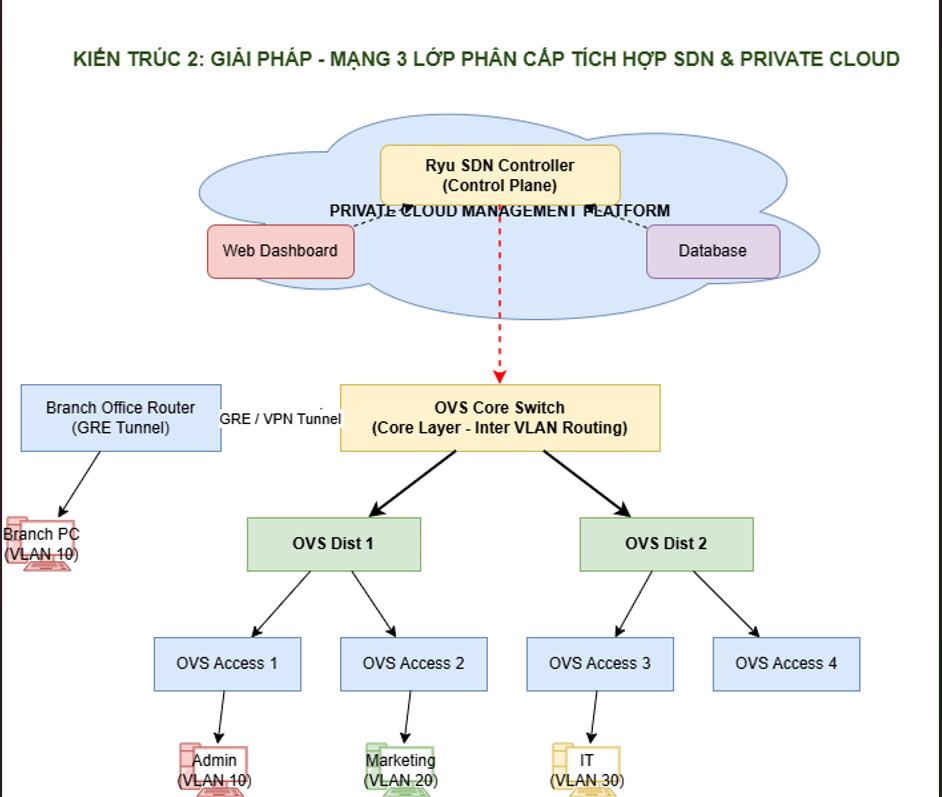
\includegraphics[width=0.9\textwidth]{image/3tier_network.png}
    \caption{Sơ đồ mô hình mạng phân tầng 3 lớp}
    \label{fig:three_tier_network_ch3}
\end{figure}

\paragraph{Đặc điểm cấu trúc}
Mô hình mạng 3 lớp là kiến trúc được thiết kế theo nguyên tắc phân cấp, chia mạng thành ba lớp: Core Layer, Distribution Layer và Access Layer, mỗi lớp có vai trò và chức năng riêng biệt.

\textbf{Các thành phần chính:}
\begin{itemize}
    \item \textbf{Core Layer (Lớp lõi):} Backbone của mạng, đảm nhận việc chuyển tiếp dữ liệu tốc độ cao giữa các Distribution Layer.
    \item \textbf{Distribution Layer (Lớp phân phối):} Thực hiện routing, filtering, QoS, aggregation, áp dụng các policy và access control list (ACL).
    \item \textbf{Access Layer (Lớp truy cập):} Kết nối trực tiếp với thiết bị đầu cuối, thực hiện VLAN assignment, port security, 802.1X authentication.
\end{itemize}

\paragraph{Ưu điểm}
\begin{enumerate}
    \item \textbf{Hiệu năng cao:} Phân tầng giúp tối ưu hóa luồng dữ liệu, giảm bottleneck và tăng throughput.
    \item \textbf{Bảo mật tốt:} Có thể áp dụng các chính sách bảo mật khác nhau cho từng lớp, dễ dàng phân đoạn mạng và kiểm soát truy cập.
    \item \textbf{Khả năng mở rộng:} Dễ dàng thêm thiết bị mới mà không ảnh hưởng đến hiệu năng tổng thể của mạng.
    \item \textbf{Quản lý tập trung:} Có thể áp dụng các chính sách quản lý thống nhất, dễ dàng giám sát và xử lý sự cố.
    \item \textbf{Tính sẵn sàng cao:} Dễ dàng triển khai các giải pháp redundancy và failover cho từng lớp.
    \item \textbf{Hỗ trợ QoS:} Có thể ưu tiên các loại traffic quan trọng, đảm bảo chất lượng dịch vụ.
    \item \textbf{Dễ dàng troubleshooting:} Cấu trúc phân tầng giúp xác định nhanh chóng vị trí xảy ra sự cố.
\end{enumerate}

\paragraph{Nhược điểm}
\begin{enumerate}
    \item \textbf{Chi phí cao:} Cần đầu tư nhiều thiết bị phần cứng cho từng lớp, thiết bị Core và Distribution thường có giá thành rất cao.
    \item \textbf{Cấu hình phức tạp:} Phải cấu hình thủ công từng thiết bị qua CLI, dễ xảy ra sai sót và không đồng nhất giữa các thiết bị.
    \item \textbf{Thời gian triển khai dài:} Cần nhiều thời gian để thiết kế, cấu hình và kiểm tra toàn bộ hệ thống.
    \item \textbf{Yêu cầu chuyên môn cao:} Cần đội ngũ kỹ thuật có kiến thức chuyên sâu về mạng để vận hành và bảo trì.
    \item \textbf{Khó thay đổi:} Khi cần thay đổi topology hoặc policy, phải can thiệp vào nhiều thiết bị, có thể gây gián đoạn dịch vụ.
    \item \textbf{Single point of failure:} Mỗi lớp có thể trở thành điểm yếu đơn lẻ, đặc biệt là Core Layer.
    \item \textbf{Khó tự động hóa:} Việc triển khai tự động rất khó thực hiện với kiến trúc truyền thống.
\end{enumerate}

\paragraph{Phù hợp với}
\begin{itemize}
    \item Doanh nghiệp vừa và lớn
    \item Trường học, bệnh viện, cơ quan chính phủ
    \item Data center, hệ thống mạng yêu cầu độ ổn định cao
    \item Môi trường có nhiều phòng ban với yêu cầu bảo mật khác nhau
    \item Hệ thống yêu cầu khả năng mở rộng và tính sẵn sàng cao
\end{itemize}

\subsection{So sánh tổng quan hai sơ đồ mạng}

\begin{table}[H]
\centering
\caption{Bảng so sánh chi tiết hai sơ đồ mạng}
\label{tab:network_comparison_detail}
\begin{tabular}{|p{4.5cm}|p{6cm}|p{6cm}|}
\hline
\textbf{Tiêu chí} & \textbf{Mạng phẳng} & \textbf{Mạng 3 tầng} \\
\hline
\hline
\textbf{Chi phí đầu tư} & Thấp (ít thiết bị, cấu hình đơn giản) & Cao (nhiều thiết bị chuyên dụng, cấu hình phức tạp) \\
\hline
\textbf{Hiệu năng} & Kém khi số lượng thiết bị lớn (broadcast storm) & Tốt với traffic phân tầng và phân đoạn hợp lý \\
\hline
\textbf{Bảo mật} & Yếu (không có segmentation) & Tốt (có segmentation và ACL theo từng lớp) \\
\hline
\textbf{Khả năng mở rộng} & Hạn chế (giới hạn broadcast domain) & Tốt (dễ dàng thêm thiết bị vào từng lớp) \\
\hline
\textbf{Quản lý} & Đơn giản nhưng không hiệu quả khi mở rộng & Phức tạp nhưng hiệu quả, có thể quản lý tập trung \\
\hline
\textbf{Tính sẵn sàng} & Thấp (khó triển khai redundancy) & Cao (dễ triển khai failover cho từng lớp) \\
\hline
\textbf{Tự động hóa} & Không hỗ trợ & Khó khăn, không có cơ chế API chuẩn \\
\hline
\textbf{Quality of Service} & Không hỗ trợ & Hỗ trợ tốt, có thể ưu tiên traffic \\
\hline
\textbf{Thời gian triển khai} & Nhanh (vài giờ đến vài ngày) & Chậm (vài tuần đến vài tháng) \\
\hline
\textbf{Yêu cầu chuyên môn} & Thấp (kiến thức cơ bản) & Cao (chuyên gia mạng có kinh nghiệm) \\
\hline
\textbf{Phù hợp} & Mạng nhỏ (<50 thiết bị) & Doanh nghiệp vừa và lớn (>100 thiết bị) \\
\hline
\end{tabular}
\end{table}

\subsection{Kết luận và lựa chọn mô hình phù hợp}

Dựa trên phân tích chi tiết ở trên, chúng ta có thể đưa ra các kết luận sau:

\paragraph{Chọn mô hình mạng phẳng khi:}
\begin{itemize}
    \item Ngân sách hạn chế, cần giải pháp chi phí thấp
    \item Quy mô mạng nhỏ (dưới 50 thiết bị)
    \item Không yêu cầu bảo mật cao
    \item Cần triển khai nhanh chóng
    \item Không có đội ngũ kỹ thuật chuyên sâu về mạng
\end{itemize}

\paragraph{Chọn mô hình mạng 3 tầng khi:}
\begin{itemize}
    \item Có ngân sách đủ để đầu tư thiết bị chất lượng cao
    \item Quy mô mạng lớn (trên 100 thiết bị)
    \item Yêu cầu bảo mật cao, cần phân đoạn mạng
    \item Cần khả năng mở rộng trong tương lai
    \item Yêu cầu tính sẵn sàng và độ tin cậy cao
    \item Có đội ngũ kỹ thuật có chuyên môn về mạng
\end{itemize}

\paragraph{Xu hướng phát triển:}
Trong bối cảnh công nghệ phát triển, các mô hình mạng hiện đại như Software Defined Networking (SDN) và Cloud Computing đang kết hợp ưu điểm của cả hai mô hình truyền thống:
\begin{itemize}
    \item \textbf{Tính linh hoạt} của mạng phẳng: Dễ dàng thay đổi cấu hình
    \item \textbf{Bảo mật và hiệu năng} của mạng 3 tầng: Phân đoạn mạng và quản lý tập trung
    \item \textbf{Tự động hóa:} Giảm thiểu can thiệp thủ công
    \item \textbf{Khả năng mở rộng:} Dễ dàng thêm thiết bị và dịch vụ mới
\end{itemize}

Việc lựa chọn mô hình mạng phụ thuộc vào nhiều yếu tố: ngân sách, quy mô, yêu cầu bảo mật, khả năng mở rộng và nguồn nhân lực kỹ thuật. Trong thực tế, nhiều tổ chức áp dụng mô hình lai (hybrid) để tận dụng ưu điểm của cả hai mô hình.

\end{document}